\chapter{Struttura della memoria centrale}
\label{cha:centralMem}

\section{Decoder e memorie}
\label{sec:decoderMemorie}

Supponiamo di voler realizzare 1 MB di RAM utilizzando un certo numero di chip: per indirizzare tale quantità di memoria servono 20 bit, quindi una scelta potrebbe essere quella di utilizzare $2^3$ chip da $2^{20-3}=2^{17}=128K$ byte. Ogni chip avrà perciò la struttura come quella in figura \ref{fig:decoderino}, con 17 bit di indirizzamento e un segnale di \textit{enable} per attivare o meno il dispositivo (e spegnerlo quando non c'è bisogno, per evitare conflitti e risparmiare preziosa energia).

\begin{figure}[!h]
\centering
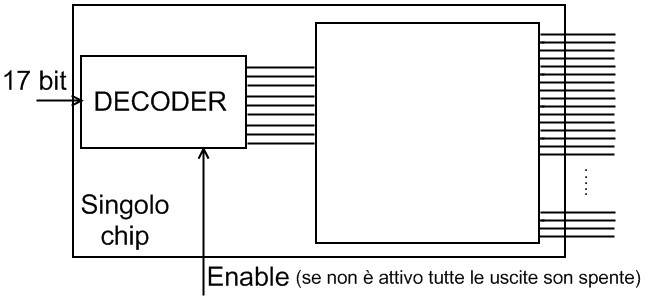
\includegraphics[width=0.65\columnwidth]{img/decoderino}
\caption{Chip da 128 KB (17 bit di indirizzamento)}
\label{fig:decoderino}
\end{figure}

All'interno del chip è presente un decoder, dispositivo a $N$ ingressi e $2^N$ uscite, una sola delle quali è attiva in un certo istante: esiste infatti una sola uscita ad '1', qualsiasi sia la configurazione d'ingresso.

Volendo, possiamo sfruttare la proprietà associativa della moltiplicazione [$x_1x_2x_3=(x_1x_2)x_3$] per costruire un decoder a $2^N$ uscite a partire da $2^{(N-K)}$ analoghi componenti con $2^K$ uscite: nell'esempio in figura \ref{fig:decoderone} si mostra come ottenere un decoder a $2^4=16$ uscite a partire da $2^{(4-2)}=4$ decoder a $2^2=4$ uscite.

\begin{figure}[!h]
\centering
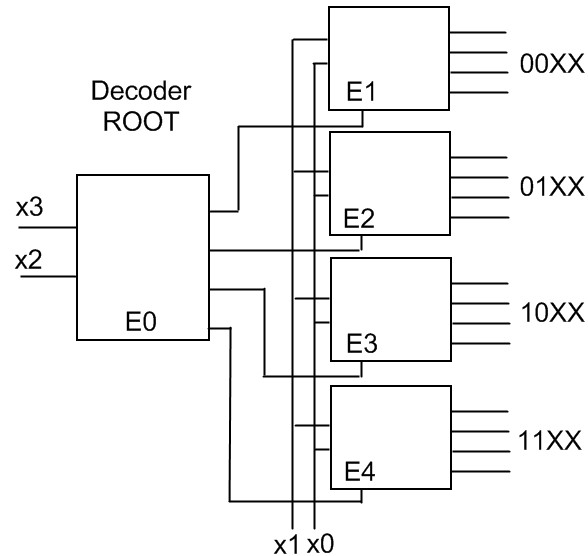
\includegraphics[width=0.55\columnwidth]{img/decoderone}
\caption{Costruzione di un decoder a $2^N$ uscite a partire da $2^{(N-K)}$ analoghi componenti con $2^K$ uscite}
\label{fig:decoderone}
\end{figure}

Il decoder \textit{root}, cioè quello di livello più alto, utilizza i due bit più significativi ($x_3x_2$) per discriminare quale dei quattro decoder "'figli'" attivare tramite il segnale di \textit{enable}: ognuno di questi, a sua volta, sceglie quale uscita far passare ad '1' in base ai bit meno significativi $ x_1x_0$.
Nell'esempio fatto ad inizio capitolo (1 MB RAM, 8 chip da 128 KB) possiamo scegliere di usare 3 bit per il decoder \textit{root} e 17 bit per ogni chip come quello in figura \ref{fig:decoderino}.

\section{Bus dati con parallelismo di $n$ byte}
\label{sec:multipliByte}

\textsf{
\textit{NOTA PRELIMINARE: in questo paragrafo faremo due esempi. Il primo, con 4 banchi (v. oltre), si riferisce ad una  architettura a 32 bit. Il Pentium, con bus dati a 64 bit, dispone di 8 banchi per poter sfruttare al massimo il suo parallelismo.}} \\


La quantità minima di informazioni normalmente indirizzabile da parte di un microprocessore è pari ad un byte, ma non è necessario che il bus dati del microprocessore abbia il parallelismo limitato a un byte. Ci si può quindi porre l'obiettivo di aumentare il parallelismo del bus al fine di trasferire più byte in un solo trasferimento, col vincolo di conservare l'indirizzabilità del singolo byte. Vogliamo cioè aumentare il \textit{throughput} del bus senza cambiare le temporizzazioni, portando il parallelismo del bus dati a $m$ byte, con $ m = 2^k$, in modo da poter trasferire fino a $2^k$ byte per ogni trasferimento. Tutto ciò è arduo da farsi all'interno di una memoria con struttura monolitica. Piuttosto, fa maggiormente al caso nostro una memoria suddivisa in più "'compartimenti'" (banchi) in grado di essere attivi indipendentemente l'uno dall'altro (a differenza di quanto permette il decoder, che accende sempre una sola uscita alla volta). Per realizzare quanto appena detto è necessario che indirizzi consecutivi appartengano a chip diversi (\textit{interleaving}); si osservi ad esempio la figura \ref{fig:bancobanchi}: essa mostra come sia possibile suddividere una memoria da 4 GB in più banchi di memoria, ognuno di dimensione inferiore (2x2 GB, 4x1 GB). Se ci raffiguriamo mentalmente la nostra memoria bidimensionale (il rettangolone con gli indirizzi scritti di fianco, tanto per intenderci) dobbiamo immaginare l'indirizzamento a partire da in basso a destra e andando prima verso sinistra e poi verso l'alto, come suggerisce la figura \ref{fig:alfaBetaBanchi}, con il primo byte nel banco 0 avente indirizzo 0, il secondo avente indirizzo 4, il terzo avente indirizzo 8 etc\ldots (se leggiamo dal basso verso l'alto, nel banco 1 avremo invece gli indirizzi 1, 5 e 9\ldots, nel banco 2 gli indirizzi 2, 6, 10\ldots e così via).

\begin{figure}[!h]
\centering
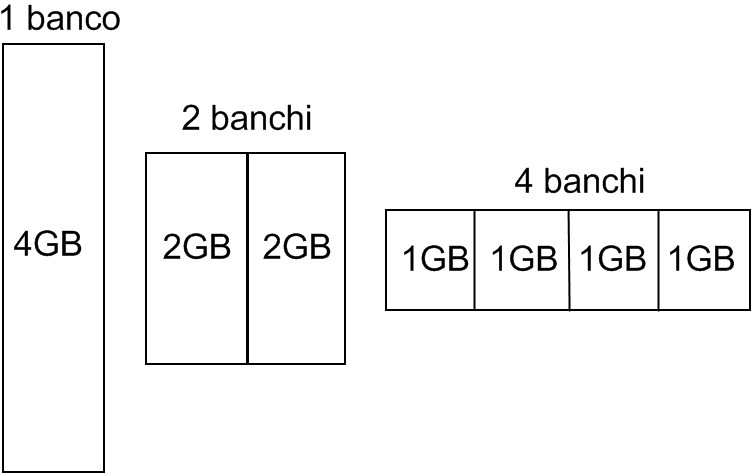
\includegraphics[width=0.5\columnwidth]{img/bancobanchi}
\caption{Frammentazione della memoria monoblocco in banchi di varie dimensioni}
\label{fig:bancobanchi}
\end{figure}

Se, come abbiamo detto poco fa, è possibile attivare i banchi indipendentemente l'uno dall'altro, sarà possibile selezionare fino a 4 byte (32 bit) a seconda se vogliamo un byte, una \textit{word} (2 byte, 2 banchi attivi), una\textit{ double word} (4 byte, 4 banchi attivi). Nell'esempio in figura \ref{fig:alfaBetaBanchi}, possiamo prendere ALFA selezionando il banco 0, mentre BETA è stata allocata ad indirizzi contigui (1-4) secondo la convenzione \textit{little endian}.

\begin{figure}[!h]
\centering
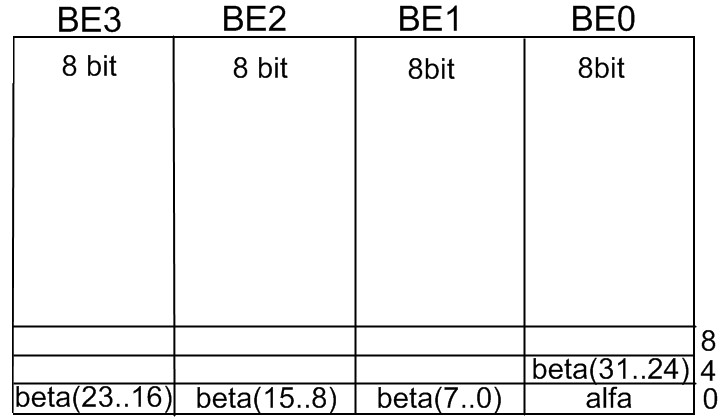
\includegraphics[width=0.65\columnwidth]{img/alfaBetaBanchi}
\caption{Divisione della memoria in banchi e allocazione delle variabili}
\label{fig:alfaBetaBanchi}
\end{figure}

I segnali che permettono di abilitare i banchi e distinguere fra i vari casi descritti sopra vengono detti \textit{bank enable} (BE). Per quanto detto fin'ora, possiamo sinteticamente affermare che il \textit{chip select} (CS) di un qualsiasi blocco di memoria mappato nella finestra di indirizzamento di 4 GB del nostro calcolatore sarà individuato da due coordinate: la finestra di offset (coordinata verticale), che si configura come il classico \textit{chip select} visto a Calcolatori L-A, e il \textit{bank enable} (BE). Il microprocessore sa dove comincia un determinato dato, quale sia la sua dimensione e il suo offset nel banco dunque è perfettamente in grado di accedervi.

\begin{figure}[!h]
\centering
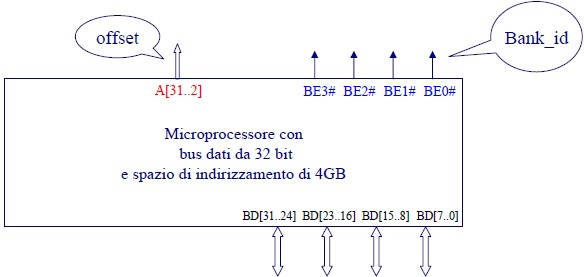
\includegraphics[width=0.75\columnwidth]{img/microMultiByte}
\caption{Struttura del bus degli indirizzi in un microprocessore con
bus dati e indirizzi di 32 bit}
\label{fig:microMultiByte}
\end{figure}

In figura \ref{fig:microMultiByte} notiamo che:
\begin{itemize}
\item i pin della CPU da interfacciare al bus dati sono suddivisi in gruppi di 8 pin (chiamati BD[\ldots]);
\item ad ogni gruppo è associato un segnale $BEi$: se è attivo, la CPU trasferisce dati sul corrispondente insieme di pin BD[\ldots];
\item ad ogni ciclo di bus il microprocessore genera un offset e attiva uno o più segnali di \textit{bank enable};
\item ogni \textit{bank enable} attivo individua una delle quattro celle da un byte associate all'offset presente sul bus degli indirizzi in posizione A[31..2]: questo byte sarà trasferito su un ben preciso byte del bus dati. Chiaramente il numero dei  \textit{bank enable} attivi dipende dal numero di byte del dato da trasferire;
\item se il dato da trasferire è composto da byte con diversi valori di offset (dato non allineato), il
microprocessore non ha scelta e dovrà effettuare più trasferimenti sul bus; in caso contrario (dato allineato) il trasferimento avviene solamente in un ciclo.
\end{itemize}

Le seguenti sono le formule per la traduzione dell'indirizzo dato in 2 coordinate e quello fisico (cioè preso "'in senso classico'") e viceversa:
\[
\begin{gathered}
IF = \text{Offset} \cdot Numero_{banchi} + BankId \\
BankId = \operatorname{MOD_{NumeroBanchi}}(IF) \\
\text{Offset} = \dfrac{IF}{Numero_{banchi}} = IF >> \log_2\left( Numero_{banchi}\right)
\end{gathered}
\]

\begin{figure}[!h]
\centering
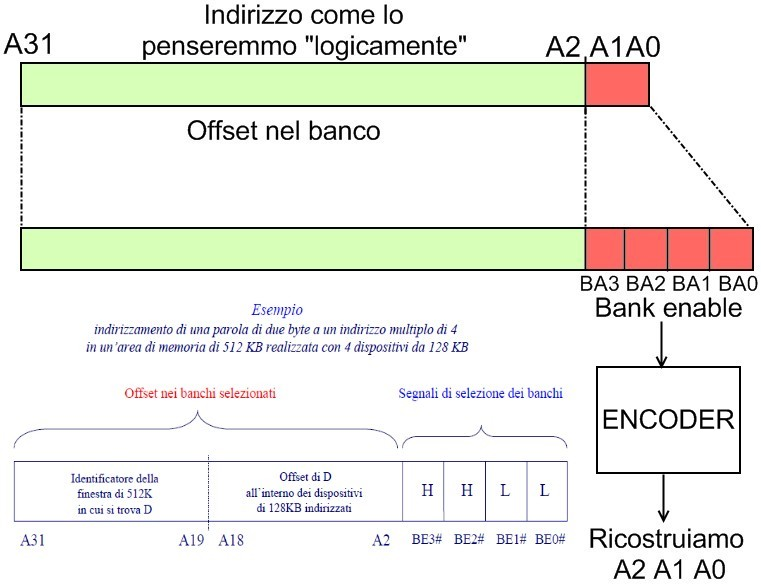
\includegraphics[width=0.85\columnwidth]{img/3234bit}
\caption{Configurazione di offset e BE nel caso di bus dati da 32 bit}
\label{fig:3234bit}
\end{figure}

In figura \ref{fig:3234bit} viene mostrata la corrispondenza fra l'array di 32 bit che indirizza i 4 GB "'in senso classico'" e la rappresentazione a 34 bit (30 di offset + 4 \textit{bank enable}) del nostro sistema a \textit{bus multibyte}. Chiaramente i 34 bit non possono viaggiare in un bus degli indirizzi da 32 bit: per questo è presente un encoder in grado di tradurre l'array dei \textit{bank enable} BE[3..0] in un numero binario di 2 bit. Allo stesso modo, nel nostro Pentium con bus dati a 64 bit (e bus degli indirizzi a 32 bit), abbiamo bisogno di un encoder che prenda in pasto gli 8 \textit{bank enable} (ogni banco occupa 512 KB) e lo traduca nei bit\footnote{Non posseduti dal microprocessore.} A2, A1 e A0 da inserire nel "'classico'" indirizzo da 32 bit (quello che daremmo in una memoria monobanco) come mostrato in figura \ref{fig:banktraduzione64}.

\begin{figure}[!h]
\centering
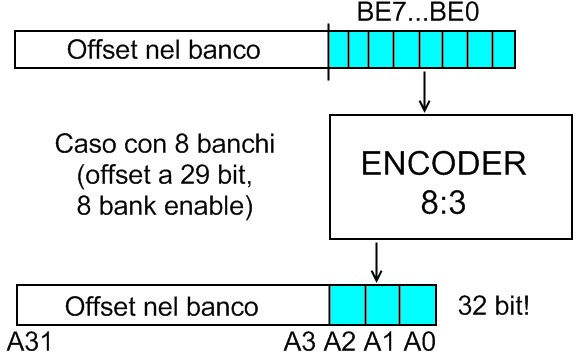
\includegraphics[width=0.5\columnwidth]{img/banktraduzione64}
\caption{Traduzione dei segnali di \textit{bank enable} nel caso a 8 banchi}
\label{fig:banktraduzione64}
\end{figure}

\section{E le periferiche?}
\label{sec:perifericheCacchio}

Per quanto riguarda le periferiche, è il \textit{bridge} che si occupa di intercettare più banchi e interfacciare correttamente il bus di I/O (8 bit) e quello dei dati (64 bit, sempre nel Pentium).
Nei trasferimenti da bus dati a bus di input/output il bridge funge infatti da multiplexer da 8 bit a 8 vie, mettendo cioè in comunicazione ciascuno degli 8 banchi del bus dati con il bus di I/O. Nei trasferimenti in direzione opposta (da bus di input/output a bus di memoria) il bridge trasferisce il contenuto del bus di I/O sui banchi del bus dati. Di conseguenza, grazie al bridge, la CPU può comunicare con il bus di I/O attraverso qualunque dei suoi banchi del bus dati: questo significa che i dispositivi interfacciati al bus di I/O possono essere mappati a qualunque indirizzo, quindi in particolare a indirizzi adiacenti. Inoltre è possibile effettuare trasferimenti in DMA di blocchi di dati contigui (come vedremo in seguito).

Per mappare le periferiche si segue dunque lo schema d'indirizzamento riportato in figura \ref{fig:perifericheBanchi}.

\begin{figure}[!h]
\centering
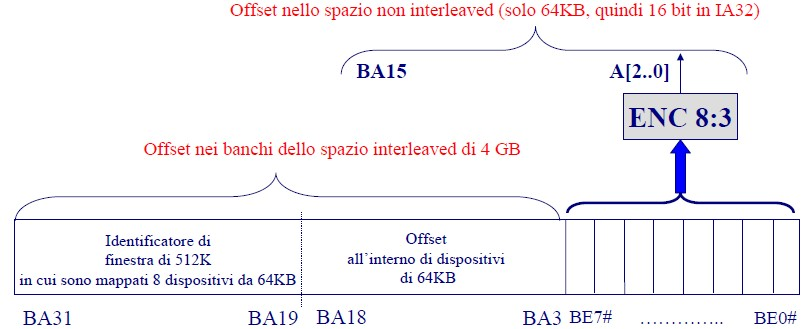
\includegraphics[width=0.85\columnwidth]{img/perifericheBanchi}
\caption{Gestione degli indirizzi in un sistema con bus dati da 64 bit e bus di I/O da 8 bit}
\label{fig:perifericheBanchi}
\end{figure} 

Si noti che è indispensabile porre ogni chip ad un indirizzo allineato (cioè multiplo della sua dimensione).

\section{Un esempio}
\label{sec:esempio}

Un sistema A basato su una CPU da 32 bit, con bus dati da 64 bit e un bus di I/O da 8 bit (separati
da un bridge), dispone di un DMAC, un PIC e una porta seriale S1 (un chip 8250).

\begin{figure}[!h]
\centering
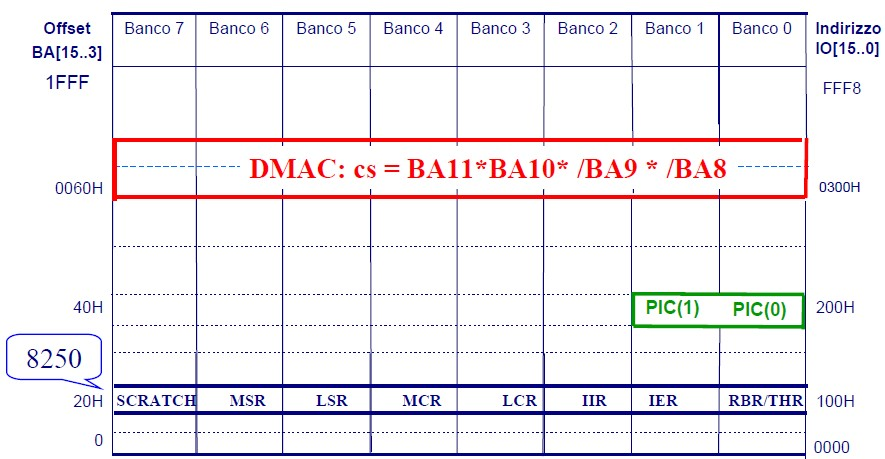
\includegraphics[width=0.95\columnwidth]{img/esempioPerifericheMappate}
\caption{Posizione dei dispositivi di Input/Output nello spazio di indirizzamento di I/O}
\label{fig:esempioPerifericheMappate}
\end{figure}

In figura \ref{fig:esempioPerifericheMappate} viene mostrata una possibile scelta di \textit{mapping} delle periferiche in I/O. Si noti la presenza di 8 banchi (ognuno da 8 KB per un totale di 64 KB di spazio di indirizzamento in I/O). A 100H è stato mappata la seriale (8 byte, si veda la figura \ref{fig:mux8vie} per uno "'zoom'" dello schema d'interfacciamento fra essa e la memoria centrale tramite il bridge), a 200H il PIC (2 byte) e a 300H il DMA Controller (16 byte): tutti gli indirizzi sono quindi allineati!
Volendo, ad esempio, accedere al registro IER, l'indirizzo sarà:
\begin{verbatim}
A15 A14 A13 A12 | A11 A10 A9 A8 | A7 A6 A5 A4 | A3 A2 A1 A0
  0   0   0   0 |   0   0  0  1 |  0  0  0  0 |  0  0  0  1

In esadecimale: 0101F
\end{verbatim}

\begin{figure}[!h]
\centering
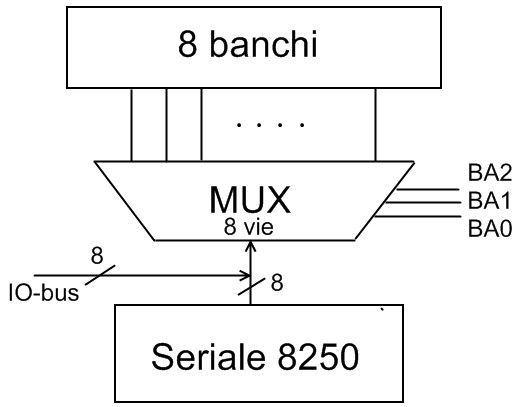
\includegraphics[width=0.75\columnwidth]{img/mux8vie}
\caption{Schema di interfacciamento fra la seriale e la memoria centrale tramite il bridge}
\label{fig:mux8vie}
\end{figure}
